\chapter{MDFT: version à symétrie radiale}

\boitemagique{Objectif}{
L'objectif de ce chapitre est de proposer une version de MDFT permettant une étude rapide et précise des systèmes à symmétrie radiale, c'est à dire l'étude de solute simples sphériques et neutres.
}

Les solutés à symétrie radiale constituent une sous catégorie très importante dans le test et le calibrage de nouvelles théories. On compte parmi eux, les gaz rares, des molécules unifiés telles que le methane ou le néopentane, représentés par un unique site Lennard-Jones ou encore des solutés historiquement utilisés dans de nombreux articles de présentations de nouvelles méthodes: les sphères dures. Une version allégée de MDFT à symétrie radiale nous permet ainsi de tester et de calibrer de nouvelles théories de façon simple et rapide.

\section{Système à symétrie radiale}

\subsubsection{La fonctionnelle à symétrie sphérique}
\begin{figure}
    \centering
	\begin{tikzpicture}
      \begin{scope}
  % coordinaten
      \coordinate (m) at (0,4,0);
      % assen
      \draw  (0,0,0) -- (0,4,0); % z
      \draw  (0,0,0) -- (4,0,0); % x
      \draw  (0,0,0) -- (0,0,4.65); % y
      % sfeer
      \draw (4,0,0) arc (0:116.5:4cm and -2cm);
      \draw (4,0,0) arc (0:90:4cm and 4cm);
      \draw (0,4,0) arc (90:206.5:2cm and 4cm);
      \node[draw, inner color=black!50, outer color=black!75, circle through={(m)}] (c) at (0,0,0) {};
      \node [ball color=purple, fill opacity=.25, circle through={(m)}] at (0,0,0) {};
      % fotosfeer
  %    \draw (3.875,0,0) arc (0:115.8:3.875cm and -1.875cm);
  %    \draw (3.875,0,0) arc (0:90:3.875cm and 3.875cm);
  %    \draw (0,3.875,0) arc (90:205.8:1.875cm and 3.875cm);
      % convenctie zone
  %    \draw (2,0,0) arc (0:116.5:2cm and -1cm);
  %    \draw (2,0,0) arc (0:90:2cm and 2cm);
  %    \draw (0,2,0) arc (90:206.5:1cm and 2cm);
      % fill

  \draw[fill=red!10] (4.00,0,0) arc (0:90:4.00 cm and 4.00 cm) -- (0,3.75,0) arc (90:0:3.75 cm and 3.75 cm) -- (4.00,0,0);
  \draw[fill=red!10] (3.75,0,0) arc (0:90:3.75 cm and 3.75 cm) -- (0,3.50,0) arc (90:0:3.50 cm and 3.50 cm) -- (3.75,0,0);
  \draw[fill=blue!10] (3.50,0,0) arc (0:90:3.50 cm and 3.50 cm) -- (0,3.25,0) arc (90:0:3.25 cm and 3.25 cm) -- (3.50,0,0);
  \draw[fill=blue!20] (3.25,0,0) arc (0:90:3.25 cm and 3.25 cm) -- (0,3.00,0) arc (90:0:3.00 cm and 3.00 cm) -- (3.25,0,0);
  \draw[fill=blue!10] (3.00,0,0) arc (0:90:3.00 cm and 3.00 cm) -- (0,2.75,0) arc (90:0:2.75 cm and 2.75 cm) -- (3.00,0,0);
  \draw[fill=red!10] (2.75,0,0) arc (0:90:2.75 cm and 2.75 cm) -- (0,2.50,0) arc (90:0:2.50 cm and 2.50 cm) -- (2.75,0,0);
  \draw[fill=red!30] (2.50,0,0) arc (0:90:2.50 cm and 2.50 cm) -- (0,2.25,0) arc (90:0:2.25 cm and 2.25 cm) -- (2.50,0,0);
  \draw[fill=red!10] (2.25,0,0) arc (0:90:2.25 cm and 2.25 cm) -- (0,2.00,0) arc (90:0:2.00 cm and 2.00 cm) -- (2.25,0,0);
  \draw[fill=blue!20] (2.00,0,0) arc (0:90:2.00 cm and 2.00 cm) -- (0,1.75,0) arc (90:0:1.75 cm and 1.75 cm) -- (2.00,0,0);
  \draw[fill=blue!50] (1.75,0,0) arc (0:90:1.75 cm and 1.75 cm) -- (0,1.50,0) arc (90:0:1.50 cm and 1.50 cm) -- (1.75,0,0);
  \draw[fill=blue!100] (1.50,0,0) arc (0:90:1.50 cm and 1.50 cm) -- (0,1.25,0) arc (90:0:1.25 cm and 1.25 cm) -- (1.50,0,0);
  \draw[fill=blue!60] (1.25,0,0) arc (0:90:1.25 cm and 1.25 cm) -- (0,1.00,0) arc (90:0:1.00 cm and 1.00 cm) -- (1.25,0,0);




  \draw[fill=  red!10] (4.00,0,0) arc (0:116.5:4.000cm and -2.000cm) -- (0,0,0.000) -- (4.000,0,0);
  \draw[fill=  red!10] (3.75,0,0) arc (0:116.5:3.750cm and -1.875cm) -- (0,0,0.000) -- (3.750,0,0);
  \draw[fill=  blue!10] (3.50,0,0) arc (0:116.5:3.500cm and -1.750cm) -- (0,0,0.000) -- (3.500,0,0);
  \draw[fill=  blue!20] (3.25,0,0) arc (0:116.5:3.250cm and -1.625cm) -- (0,0,0.000) -- (3.250,0,0);
  \draw[fill=  blue!10] (3.00,0,0) arc (0:116.5:3.000cm and -1.500cm) -- (0,0,0.000) -- (3.000,0,0);
  \draw[fill=  red!10] (2.75,0,0) arc (0:116.5:2.750cm and -1.375cm) -- (0,0,0.000) -- (2.750,0,0);
  \draw[fill=  red!30] (2.50,0,0) arc (0:116.5:2.500cm and -1.250cm) -- (0,0,0.000) -- (2.500,0,0);
  \draw[fill=  red!10] (2.25,0,0) arc (0:116.5:2.250cm and -1.125cm) -- (0,0,0.000) -- (2.250,0,0);
  \draw[fill=  blue!20] (2.00,0,0) arc (0:116.5:2.000cm and -1.000cm) -- (0,0,0.000) -- (2.000,0,0);
  \draw[fill=  blue!50] (1.75,0,0) arc (0:116.5:1.750cm and -0.875cm) -- (0,0,0.000) -- (1.750,0,0);
  \draw[fill=  blue!100] (1.50,0,0) arc (0:116.5:1.500cm and -0.750cm) --  (0,0,0.000) -- (1.500,0,0);
  \draw[fill=  blue!60] (1.25,0,0) arc (0:116.5:1.250cm and -0.625cm) -- (0,0,0.000) -- (1.250,0,0);




  \draw[fill=red!10](0,4.00,0) arc (90:206.5:2.000cm and 4.00cm) -- (0,0,0) -- (0,4.00,0);
  \draw[fill=red!10] (0,3.75,0) arc (90:206.6:1.875cm and 3.75cm) -- (0,0,0) -- (0,3.75,0);
  \draw[fill=blue!10] (0,3.50,0) arc (90:206.5:1.750cm and 3.50cm) -- (0,0,0) -- (0,3.50,0);
  \draw[fill=blue!20] (0,3.25,0) arc (90:206.5:1.625cm and 3.25cm) -- (0,0,0) -- (0,3.25,0);
  \draw[fill=blue!10] (0,3.00,0) arc (90:206.5:1.500cm and 3.00cm) -- (0,0,0) -- (0,3.00,0);
  \draw[fill=red!10] (0,2.75,0) arc (90:206.6:1.375cm and 2.75cm) -- (0,0,0) -- (0,2.75,0);
  \draw[fill=red!30] (0,2.50,0) arc (90:206.5:1.250cm and 2.50cm) -- (0,0,0) -- (0,2.50,0);
  \draw[fill=red!10] (0,2.25,0) arc (90:206.5:1.125cm and 2.25cm) -- (0,0,0) -- (0,2.25,0);
  \draw[fill=blue!20] (0,2.00,0) arc (90:206.5:1.000cm and 2.00cm) -- (0,0,0) -- (0,2.00,0);
  \draw[fill=blue!50] (0,1.75,0) arc (90:206.6:0.875cm and 1.75cm) -- (0,0,0) -- (0,1.75,0);
  \draw[fill=blue!100] (0,1.50,0) arc (90:206.5:0.750cm and 1.50cm) -- (0,0,0) -- (0,1.50,0);
  \draw[fill=blue!60] (0,1.25,0) arc (90:206.5:0.625cm and 1.25cm) -- (0,0,0) -- (0,1.25,0);


      % solute
      \draw[gray, fill=gray] (1,0,0) arc (0:116.5:1cm and -0.5cm) -- (1,0,0) arc (0:90:1cm and 1cm) -- (0,1,0) arc (90:206.5:0.5cm and 1cm);
      \draw[black] (1,0,0) arc (0:116.5:1cm and -0.5cm);
      \draw[black] (1,0,0) arc (0:90:1cm and 1cm);
      \draw[black] (0,1,0) arc (90:206.5:0.5cm and 1cm);
	
	\end{scope}
    \begin{scope}[shift={(5, -3)}]
		\begin{axis}[colorbar, colormap name={RdBu-11},
        point meta min = 0,
        point meta max = 2,
        hide x axis,
        hide y axis]

		\end{axis}
	\end{scope}
%    \begin{scope}[shift{(-1.5, 2.8)}]
%    \begin{axis}[colorbar,colormap name={RdBu-11},
%      point meta min = 0,
%      point meta max = 2,
%      hide y axis,
%      hide x axis,
%    ]
%	  \end{axis}
%    \end{scope}
  \end{tikzpicture}
	\caption{blablabla}
    \label{fig:symmetrie_radiale}
\end{figure}

Dans cette version de la théorie, le soluté est unique et plongé au milieu d'une infinité de solvant (voir figure \ref{fig:symmetrie_radiale}), contrairement à la théorié présentée au chapitre XXXX qui est périodique et que l'on nommera la version 3D. Du fait de la symétrie radiale, le solvant forme ensuite des couches de densité comme montré en figure \ref{fig:symmetrie_radiale} jusqu'à tendre vers la densité bulk. La densité du solvant dépend uniquement de la distance $r$ par rapport au soluté, (le centre du repère), ce qui nous permet de réécrire la fonctionnelle de la façon suivante:

\begin{eqnarray}
F[\rho(r)] &=& F_{id}[\rho(r)] + F_{ext}[\rho(r)] + F_{exc}[\rho(r)] \\
F_{id}[\rho(r)]&=&k_{B}T\int_{0}^{\inf}[\rho(r)ln(\frac{\rho(r)}{\rho_{0}})-\rho(r)+\rho_{0}]V(r)\; dr \\
F_{ext}[\rho(r)]&=& \int_{0}^{\inf}\rho(r)v_{ext(r)}V(r)\; dr \\
F_{exc}[\rho(r)]&=& k_{B}T\int_{0}^{\inf}\Delta\rho(r_1) \int_{0}^{\inf}\Delta\rho(r_2)C_s(|r_2-r_1|)V(r_2)V(r_1)  \; dr_2 dr_1
\end{eqnarray}
avec $V(r)$, le volume de la coquille de rayon $r$, soit:
\begin{equation}
V(r)=4\pi r^2dr
\end{equation}

\subsubsection{Convolution à symétrie sphérique}
Comme dans la version 3D, la convolution entre $\Delta\rho(r_2)$ et $C_s(|r_2-r_1|)$ sera calculée dans l'espace de Fourier. Cependant, comme le système est à symétrie radiale, il à fallu remplacer les transformée de Fourier par des transformées de Hankel que l'on nommera HT. Les formule des transformée de Hankel directes est inverses sont les suivantes:
\begin{eqnarray}
\widehat{f}(k)&=&4\pi\int_{0}^{\inf}f(r)\frac{sin(kr)}{kr}r^2dr\\
f(r)&=&\frac{1}{2\pi^2}\int_{0}^{\inf}\widehat{f}(k)\frac{sin(kr)}{kr}k^2dk
\end{eqnarray}

%y(k) = 4 pi int _0 ^\infty  y(r) sin(kr)/(kr) r^2 dr
%	 *
%y(r) = 1/(2 pi^2) int _0 ^\infty y(k) sin(kr)/(kr) k^2 dk


Les détails de l'implémentation sont disponibles au paragraphe \ref{sec:hankel_implementation}. 

\subsubsection{Le solvant}
Pour que le système soit à symétrie radiale, nous avons également du nous affranchir de l'orientation du solvant. Pour rappel, notre modèle d'eau, le modèle SPC/E est composé de trois atomes dont deux, les hydrogènes représentés uniquement par des charges partielles. Pour nous affranchir des orientations du solvant, il nous suffit ainsi de nous limiter aux composés neutres.

\section{Implémentations}
La théorie à ensuite été implémentée en c++ dans un code séquentiel d'un peu moins de 3000 lignes. Comme le montre l'image \ref{fig:symmetrie_radiale} la densité du solvant ne dépend que de la distance entre la position dans l'espace étudiée et le centre du soluté. Au delà d'une certaine distance, le solvant n'est plus perturbé par le soluté, et redeviens homogène de densité bulk. Le système est donc représenté par un ensemble de point régulièrement répartis entre le centre du système et une distance suffisamment grande pour atteindre le solvant homogène. Le nombre de point et la taille du système sont fournis en entrée par l'utilisateur.


\subsubsection{Les transformées de Hankel}
\label{sec:hankel_implementation}
Les transformées de Hankel ayant été implémentées spécialement pour cette version, il à été possible d'utiliser différentes astuces pour améliorer la convergence et la rapidité du calcul.
Suite aux premiers tests, il est rapidement apparu qu'une instabilité apparaissaient à grande distance du soluté. Cette instabilité s'est révélée être causé par le faible nombre de points dans l'espace de Hankel autour de zéro. Nous avons donc considérablement augmenté ce nombre de points. En effet, quelques que soit le nombre de points dans l'espace direct, l'espace inverse est composé de 100 000 points régulièrement espacés allant de 0 à 250 $\text{\AA}^{-1}$. Les transformés de Hankel étant de complexité $O(n_{direct}*n_{inverse})$,  la multiplication du nombre de points dans l'espace inverse à donc d'autant multiplié le temps de calculs car plus de 90\% du temps de calcul global est consacré aux transformées de Hankel.

Cette version, utilisant une très faible quantité de mémoire, il à été possible d'utiliser une autre astuce afin de diminuer le temps de calcul. A chaque itération, la transformée de Hankel se fait selon la même double boucle r, k. Seule les fonctions $f(r)$ et $\widehat{f}(k)$ vont varier. Il à donc été possible de mettre en mémoire le résultat de la partie la plus coûteuse du calcul soit $4\pi\frac{sin(kr)}{kr}r^2dr$. L'algorithme résultant est disponible en annexe XXXXX. Cette astuce, possible dans cette version car l'impacte mémoire est très faible, permet de diminuer le temps de calcul global par 10. Il est certainement possible d'améliorer encore cette partie, mais devant le faible coût mémoire et le faible temps de calcul obtenus, il n'est pas paru nécessaire d'aller plus loin.


\section{Résultats}
\subsubsection{\'Energies libres de solvatations}

%\begin{tikzpicture}
%   \begin{axis}[
%      height=12cm,
%      width=15cm,
%      grid=major,
%      grid style={dotted},
%      colormap/jet,
%      mesh/ordering=x varies,
%      mesh/cols=20,]
%      \addplot3[surf] file {test.csv};
%      \end{axis}
%\end{tikzpicture}


\subsubsection{Profiles de densités}
\subsubsection{Temps de calculs}

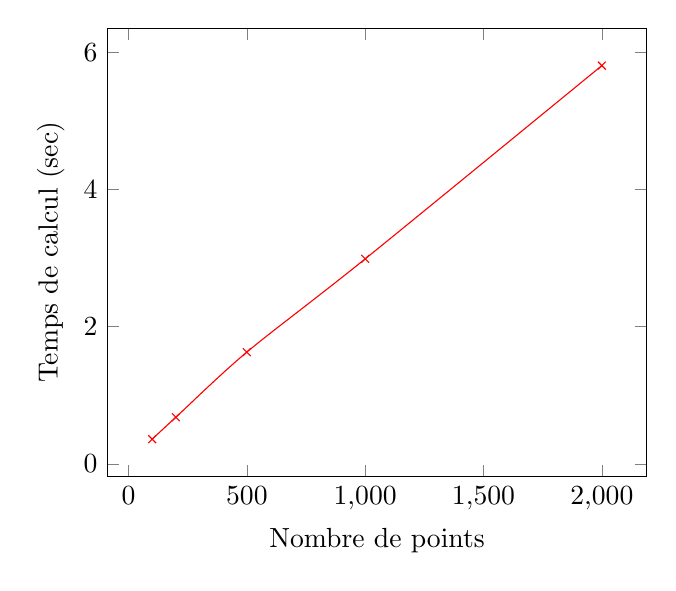
\begin{tikzpicture}
    \begin{axis}[
        xlabel=Nombre de points,
        ylabel=Temps de calcul (sec)]
    \addplot[smooth,color=red,mark=x]
        plot coordinates {
            (100,0.36)
            (200,0.68)
            (500,1.63)
            (1000,2.99)
            (2000,5.81)
        };
    \end{axis}
    \end{tikzpicture}


\begin{table}[!htbp]
  \begin{tabular}{ l c c}
    \hline & \\[-1em]\hline
    N   & HRF  & HRF + bridge \\
    \hline
    100     & 0.36 & 0.50 \\
    200     & 0.68 & 1.05 \\
    500     & 1.63 & 2.33 \\
   1000     & 2.99 & 4.86 \\
   2000     & 5.81 & 9.10 \\
    \hline & \\[-1em]\hline
  \end{tabular}
  \caption{Temps en seconds nécessaire pour générer le profil de solvatation et l'énergie libre de solvatation avec la version à gémoétrie sphérique de MDFT en fonction du nombre de points}
  \label{tab:times}
\end{table}




\begin{tikzpicture}
\begin{axis}[
    enlarge x limits=.02,
    enlarge y limits=.02,
    minor tick num=4,
    xticklabel style={/pgf/number format/fixed},% exponential axis notation looks bad in this case
    colorbar,
    scatter/use mapped color={%
      draw=mapped color,
      fill=mapped color
    }]
    \addplot[
      scatter,
      scatter src=explicit,
      only marks,
      mark=square*,
    ] file{test.csv};
  \end{axis}
\end{tikzpicture}

\begin{tikzpicture}
\begin{axis}[grid=major,view={210}{30}]
\addplot3+[mesh,scatter] table {test.csv};
\end{axis}
\end{tikzpicture}



\begin{tikzpicture}
  \begin{axis}[view={0}{90}, clip = false, grid=major, xlabel=$\sigma$, ylabel=$\epsilon$]

    \addplot +[no markers,
    raw gnuplot,
    contour prepared,
    ] gnuplot {
    %                set samples 50, 50;
    %                set isosamples 51, 51;
    set contour base;
    %                set cntrparam levels incremental -4,0.25,4;
    set cntrparam levels 15
    set style data lines;
    set sgrid3d 50, 50;
    splot "test.csv" u 1:2:3 w l ;
    };

  \end{axis}
\end{tikzpicture}


